
%
%  $Description: Author guidelines and sample document in LaTeX 2.09$ 
%
%  $Author: ienne $
%  $Date: 1995/09/15 15:20:59 $
%  $Revision: 1.4 $
%

\documentclass[times, 10pt,twocolumn]{article} 
\usepackage{epsfig}
\usepackage{latex8}
\usepackage{times}

%\documentstyle[times,art10,twocolumn,latex8]{article}

%------------------------------------------------------------------------- 
% take the % away on next line to produce the final camera-ready version 
\pagestyle{empty}

%------------------------------------------------------------------------- 
\begin{document}

\title{User-level Grid Monitoring with Inca 2}

\author{Shava Smallen, Kate Ericson, and Jim Hayes \\
San Diego Supercomputer Center\\ University of California, San Diego\\ 
9500 Gilman Drive, La Jolla, CA 92093-0505, USA\\ 
\{ssmallen,kericson,jhayes\}@sdsc.edu\\
}

\maketitle
\thispagestyle{empty}

%1.  Motivate and differentiate the Grid monitoring Inca does
%2. Describe Inca 2 design and its benefits
%3. Illustrate that Inca 2 design is mature and being used in production by
%several Grids
%4. Be different from Inca 1 paper

\begin{abstract}
User-level Grid monitoring is valuable, how it relates to other Grid
monitoring,  and what are its implementation challenges.
Inca 1 good but had limitations.  In this paper, we introduce Inca 2 and
describe its features and architecture.  We then show a few use cases for Inca
is being deployed on TeraGrid and XXX?  System impact results and performance
results.  Finally, we discuss our future work.  
\end{abstract}

%------------------------------------------------------------------------- 
\Section{Introduction}

Grid monitoring is x, y, and z.  Describe the stakeholders.

User-level Grid monitoring is x and is valuable.  

However, implementing user-level Grid monitoring has challenges.  List.

Inca 1~\cite{inca1} first addressed this but had limitations.  We learned
lessons from our TeraGrid deployment.  This motivated our development of a new
version of Inca.

~\newpage
~\newpage
~\newpage
~\newpage

%------------------------------------------------------------------------- 
\Section{Design and Implementation}

Features list.

Differences with Inca 1 table? 

Overview of all architecture components -- arch picture

The core of the Inca architecture (shown in Figure 1) is formed by two
components: the agent and the depot.  The agent controls the execution of the
Inca installation, while the depot provides data storage. All Inca components
use SSL to communicate.

\begin{figure}[Htb]
  \centering
  \mbox{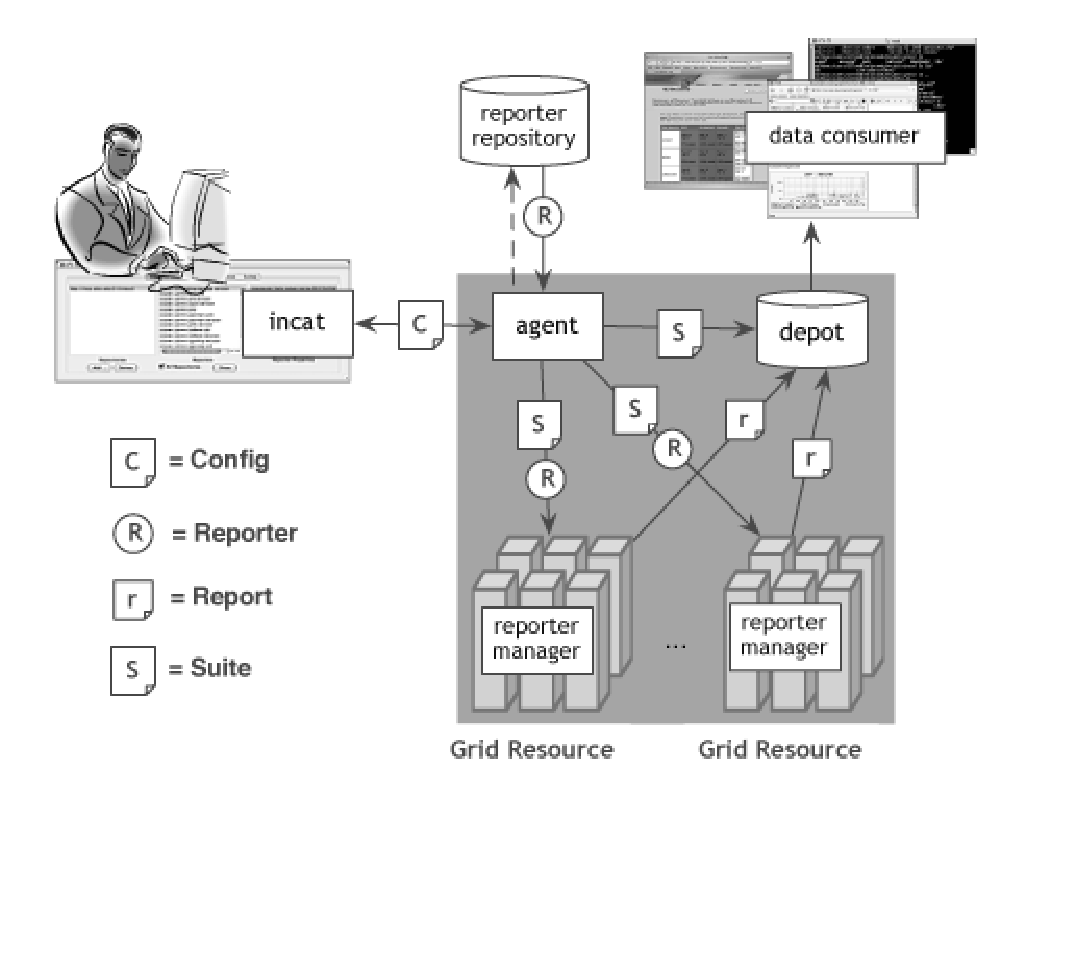
\epsfig{file=arch.eps, width=\columnwidth}}
  \caption{\label{arch_fig} Inca architecture.}
\end{figure}

The Inca agent is a server that implements the configuration specified by the
Inca administrator.  After determining which Inca tests should be executed on
each resource, the agent stores this configuration information in the depot.
It then stages and launches a dependent component, called a reporter manager,
on each resource using either SSH or Globus [13].  Once a reporter manager
contacts its agent, the agent transmits Inca tests to execute, along with
their dependencies, configuration and schedule of execution. 
  
The Inca reporter manager is a lightweight process responsible for managing
the schedule and execution of Inca tests, called reporters, on a single
resource. The reporter manager receives reporter updates and dependencies
(e.g., Inca Perl APIs or source code) from the agent along with requests for
reporter scheduling changes.  Running under a regular user account, the
reporter manager executes reporters on-demand or using an internal cron
scheduler, and sends reports to the depot for archiving. The reporter
manager monitors reporter system usage and enforces limits (e.g., wall clock
time, CPU time, memory).  System usage information is sent to the depot with
each report. 


Each Inca reporter is an executable program that tests or measures some
aspect of a system or installed software.   Reporter executables are
designed to be easy to produce and can be run outside of the Inca system
(e.g., by a system administrator).  A reporter could be a simple Globus
gatekeeper ping test (see Figure 2) or a more complex Grid application
benchmark.  Reporters must support certain command line options and produce
XML according to the Inca reporter schema.  The reporter schema requires a
header describing the context of the reporter execution (e.g., reporter
name, arguments, working directory, timestamp) and a body containing the
results expressed as any XML sequence. This flexible body schema enables
reporters to express a wide variety of information.  Today, we have three
standard body schemas to express software version information, software
functionality or service tests results, and usage information.  We provide
Perl APIs to handle much of the effort of writing reporters.  Most current
reporters use these APIs and consist of fewer than 30 lines of code.  

The Inca agent retrieves reporters from collections called reporter
repositories, that consist of reporters, required packages and libraries,
and a catalog file. Repository contents are accessible using a URL and can
be shared across multiple Inca deployments. The Inca team publishes a
reporter repository that contains reporters developed for TeraGrid.  

The Inca depot server is responsible for storing configuration information
and the data produced by reporters. The depot maintains a relational
database via Hibernate [14] so that it can use a variety of databases.  The
depot provides full archiving of reporter output and structures its schema
to reduce redundant data.  Data can be queried using SQL queries. Predefined
queries exist to return the latest report instances of a suite, a single
report instance, or a report history.  A Web services interface is also
available to provide unauthenticated query access to data.  

To configure reporter execution, an Inca administrator launches a GUI tool,
called incat.  Incat allows the administrator to choose which resources to
monitor and which reporters to deploy to those resources.  For each
reporter, the administrator can specify the resources to run on,
command-line arguments, the runtime environment, the frequency of execution,
and resource limits. The Inca administrator may also group related reporters
into suites that can be shared across different Inca deployments.  This can
be useful to determine interoperability among Grids or to determine whether
an application's requirements are being fulfilled on a Grid.

The Inca data consumer is a Web application that queries the Inca depot for
data and displays it in a user-friendly format.  The data consumer is
packaged with Jetty [15] so that pages can be served immediately without
deploying Tomcat [16].  A set of JSP tags and pages query the Inca depot for
data (returned as XML) and a set of XSL stylesheets format the data as HTML.

~\newpage
~\newpage
~\newpage
~\newpage
%------------------------------------------------------------------------- 

\Section{Use Cases}

\SubSection{TeraGrid}
~\newpage
~\newpage

\SubSection{GrASP}
~\newpage

\SubSection{Other uses}
~\newpage
%------------------------------------------------------------------------- 
\Section{Future Work}
~\newpage

%------------------------------------------------------------------------- 
\Section{Summary}

~\newpage

%------------------------------------------------------------------------- 
\bibliographystyle{latex8}
\bibliography{paper}

\end{document}

